\documentclass[11pt]{article}
\usepackage[margin=1in]{geometry}
\usepackage{booktabs}
\usepackage{amsmath}
\usepackage{amssymb}
\usepackage{graphicx}
\usepackage[colorlinks=true,urlcolor=blue]{hyperref}

\title{Reward-Tilted Posterior Guidance for Discrete Diffusion\\
\large Experimental log: QM9 property guidance}
\author{}
\date{2026-08-01}

\begin{document}
\maketitle

\section{Method}
\label{sec:method}

The reverse posterior marginalizes over the clean sequence,
\begin{equation}
q(\mathbf{x}_{t-1} \mid \mathbf{x}_t)
  = \mathbb{E}_{\mathbf{x}_0 \sim q(\mathbf{x}_0 \mid \mathbf{x}_t)}
    \left[ q(\mathbf{x}_{t-1} \mid \mathbf{x}_t, \mathbf{x}_0) \right],
\end{equation}
which we importance-sample using the model's denoiser
$p_\theta(\mathbf{x}_0 \mid \mathbf{x}_t)$ as the proposal. Because the forward
noising process is shared between $q$ and $p_\theta$,
\begin{equation}
\frac{q(\mathbf{x}_0 \mid \mathbf{x}_t)}{p_\theta(\mathbf{x}_0 \mid \mathbf{x}_t)}
  = \frac{q(\mathbf{x}_0)}{p_\theta(\mathbf{x}_0)}
    \cdot \frac{p_\theta(\mathbf{x}_t)}{q(\mathbf{x}_t)},
\end{equation}
and the second factor does not depend on $\mathbf{x}_0$, so it cancels under
normalization. Defining the reward-tilted target
$q(\mathbf{x}_0) \propto p_\theta(\mathbf{x}_0)\exp(\lambda r(\mathbf{x}_0))$
leaves the importance ratio equal to $\exp(\lambda r(\mathbf{x}_0))$, giving
\begin{equation}
q(\mathbf{x}_{t-1} \mid \mathbf{x}_t)
  \approx \sum_{n=1}^{N} w_n \, q(\mathbf{x}_{t-1} \mid \mathbf{x}_t, \mathbf{x}_0^{(n)}),
  \qquad
  w_n = \frac{\exp(\lambda r(\mathbf{x}_0^{(n)}))}
             {\sum_{m=1}^{N}\exp(\lambda r(\mathbf{x}_0^{(m)}))},
\label{eq:mixture}
\end{equation}
with $\mathbf{x}_0^{(n)} \sim p_\theta(\mathbf{x}_0 \mid \mathbf{x}_t)$.

\paragraph{Relation to discriminator guidance.}
Discriminator guidance fills the same slot with a \emph{learned} density ratio,
using $D_\phi(\mathbf{x}_0)/(1 - D_\phi(\mathbf{x}_0)) \approx
q(\mathbf{x}_0)/p_\theta(\mathbf{x}_0)$ from a discriminator trained to separate
data from model samples. Our method obtains the same ratio in closed form by
\emph{defining} the target as a reward tilt, so nothing has to be trained. This
is also the key practical difference from D-CBG: the reward sees \emph{clean}
$\mathbf{x}_0$ samples, so it never needs to be robust to noised inputs, and
each denoising step costs one network forward (the same as unguided sampling)
plus $N$ CPU-side RDKit evaluations.

\paragraph{Sampling the mixture.}
Equation~\eqref{eq:mixture} is a mixture over \emph{full sequences}, and a
mixture of factorized distributions is not itself factorized. Three variants
are implemented, forming a ladder of approximations:
\begin{itemize}
  \item \textbf{exact} --- draw $n^\star \sim \mathrm{Cat}(w)$, then
        $\mathbf{x}_{t-1} \sim q(\cdot \mid \mathbf{x}_t, \mathbf{x}_0^{(n^\star)})$.
        Samples Eq.~\eqref{eq:mixture} without further approximation and
        preserves correlations across positions.
  \item \textbf{marginal} --- average the $N$ \emph{normalized} posteriors and
        sample positions independently. Exact per-position marginals, no
        correlations.
  \item \textbf{aggregate\_x0} --- substitute the weighted histogram
        $\bar{\mathbf{x}}_0$ of the $N$ candidates for $\mathbf{x}_0$ in the
        posterior and normalize once. This is the form discriminator guidance
        uses; it coincides with \textbf{marginal} for absorbing-state diffusion,
        whose posterior normalizer does not depend on $\mathbf{x}_0$, and
        differs slightly for uniform diffusion.
\end{itemize}
Note that \textbf{aggregate\_x0} reduces to the base sampler as $N \to \infty$
at $\lambda = 0$, since $\bar{\mathbf{x}}_0$ is then an unbiased Monte Carlo
estimate of $\mathbf{x}_\theta$. \textbf{exact} does not, at any $N$ --- but
that is because the base sampler is itself the factorized projection of the true
reverse step, which \textbf{exact} samples exactly whenever the weights are
uniform. The discussion after Table~\ref{tab:headline} makes this precise.

\section{Setup}

Base model: \texttt{kuleshov-group/udlm-qm9} (UDLM, uniform diffusion,
\texttt{parameterization=d3pm}), loaded from HuggingFace with no local
fine-tuning. Sequence length 32, 32 sampling steps, \texttt{use\_cache=False},
seed 1. Rewards are computed with RDKit on decoded SMILES; candidates RDKit
cannot parse receive $r = 0$, which is the minimum of both QED and ring count
and therefore also penalizes invalidity. Every configuration below shares this
base model, so differences are attributable to the guidance mechanism alone.

\paragraph{Metric conventions.}
The paper's Table 5 reports raw \emph{counts} out of 1024 generated samples
(\texttt{Valid} $= 994.8$ means 994.8 of 1024 parsed), and its \texttt{Mean}
column is the property averaged over the \emph{novel} sequences only. The
repository's evaluation code instead stores fractions, and takes
\texttt{Unique} and \texttt{Novel} as fractions \emph{of the valid set} rather
than of all samples. The two are consistent once converted: our unguided
reference produces 1002/1024 valid and 125 novel with a novel QED mean of
0.465, against the paper's UDLM validity of $1013.6$ and data QED of $0.47$.
Tables~\ref{tab:modes} and \ref{tab:lambda} below are recorded in the
repository's percentage convention because that is what the runs printed;
\texttt{scripts/make\_results\_table.py} converts to the paper's counts, so the
generated \texttt{sweep\_table} files are the ones to compare against Table 5.

\section{Which mixture-sampling variant to use}
\label{sec:modes}

Table~\ref{tab:modes} compares the three variants at $N = 10$ on 512 samples.
ESS is the effective sample size $1/\sum_n w_n^2$ of the importance weights
averaged over the batch, reported at the final step; $\mathrm{ESS} = N$ means
uniform weights and $\mathrm{ESS} = 1$ means the mixture collapsed onto a
single candidate.

\begin{table}[h]
\centering
\caption{Mixture-sampling variants, QED reward, $N=10$, 512 samples.}
\label{tab:modes}
\begin{tabular}{llrrrrrr}
\toprule
Variant & $\lambda$ & Valid \% & Unique \% & Novel \% & QED mean & Novel QED mean & ESS \\
\midrule
aggregate\_x0 & 0   & 96.68 & 100.00 & 7.27  & 0.469 & 0.460 & 10.00 \\
\midrule
exact         & 50  & 85.55 & 99.09  & 25.80 & 0.511 & 0.512 & 4.29 \\
marginal      & 50  & 84.18 & 99.77  & 22.97 & 0.501 & 0.484 & 4.90 \\
aggregate\_x0 & 50  & 95.31 & 99.80  & 9.02  & 0.487 & 0.451 & 4.63 \\
\bottomrule
\end{tabular}
\end{table}

Two findings drive the choice of default. First, \textbf{exact} attains the
largest QED gain ($0.469 \to 0.511$) but costs roughly 11 points of validity,
whereas \textbf{aggregate\_x0} keeps validity essentially at the unguided level
(96.7\,\% $\to$ 95.3\,\%) for a smaller QED gain. Second, and more
diagnostically, \textbf{exact} at $\lambda = 0$ does \emph{not} recover the
unguided sampler: it reaches only 61.7\,\% validity (128-sample run,
Table~\ref{tab:lambda}) against 96.7\,\% for \textbf{aggregate\_x0}. Committing
each step to a single sampled $\mathbf{x}_0$ injects the denoiser's sampling
noise into the trajectory, and at $N = 10$ that cost outweighs the extra
fidelity to Eq.~\eqref{eq:mixture}. Subsequent experiments therefore fix
\textbf{aggregate\_x0} and raise $N$ to 30.

\emph{This conclusion is superseded.} Both findings survive as observations at
$N = 10$, but the inference drawn from them does not: at $N = 100$--$500$ and
$\lambda = 5000$, \textbf{exact} matches \textbf{marginal} on validity and gives
the best novel QED and the highest novel count in this report. The validity cost
identified here is real but is repaired by the tilt itself, for the reason given
after Table~\ref{tab:headline}. Read this section as the record of why
\textbf{aggregate\_x0} became the default, not as a live recommendation.

\section{Exploratory $\lambda$ sweeps}

Table~\ref{tab:lambda} records the first sweeps, run with \textbf{exact} and
$N = 10$ on only 128 samples. They establish that the tilt does what the
derivation says --- QED rises monotonically in $\lambda$ --- but the sample
size is too small to resolve the ring-count trend, where the standard error of
the mean is roughly $0.1$.

\begin{table}[h]
\centering
\caption{$\lambda$ sweeps, \textbf{exact} variant, $N=10$, 128 samples each.
Underpowered; superseded by the runs in Table~\ref{tab:modes} and the sweep
described in Section~\ref{sec:pending}.}
\label{tab:lambda}
\begin{tabular}{llrrrr}
\toprule
Reward & $\lambda$ & Valid \% & Novel \% & Property mean & Property median \\
\midrule
QED        & 0   & 61.72 & 30.38 & 0.476 & 0.486 \\
QED        & 10  & 87.50 & 22.32 & 0.493 & 0.488 \\
QED        & 50  & 82.03 & 28.57 & 0.520 & 0.520 \\
QED        & 200 & 81.25 & 34.62 & 0.530 & 0.538 \\
\midrule
ring count & 0   & 61.72 & 30.38 & 1.608 & 1.000 \\
ring count & 2   & 77.34 & 33.33 & 1.788 & 2.000 \\
ring count & 10  & 85.16 & 36.70 & 1.651 & 1.000 \\
\bottomrule
\end{tabular}
\end{table}

The non-monotone ring-count column is consistent with weight degeneracy: ring
count is integer-valued, so a unit difference in reward gives a weight ratio of
$e^{\lambda}$, and at $\lambda = 10$ that is $\approx 2.2 \times 10^4$. The
mixture then collapses onto whichever single candidate happens to score
highest. This is what motivated logging ESS.

\section{The $(N, \lambda)$ grid}
\label{sec:grid}

Table~\ref{tab:grid} is the main result so far: \texttt{aggregate\_x0}, 128
samples per cell, guidance active over the whole trajectory. Counts follow the
paper's convention, and \emph{novel QED} is the paper's \texttt{Mean} column
(property averaged over novel sequences only).

\begin{table}[h]
\centering
\caption{$(N, \lambda)$ grid, \texttt{aggregate\_x0}, 128 samples per cell.
Novel QED is the metric comparable to Table 5 of the paper. The reference rows
are the QM9 training set and our unguided sampler at 1024 samples.}
\label{tab:grid}
\begin{tabular}{rrrrrrr}
\toprule
$N$ & $\lambda$ & Valid & Unique & Novel & QED mean & Novel QED mean \\
\midrule
\multicolumn{2}{l}{QM9 data (133,885)} & 133,885 & 133,885 & 133,885 & 0.465 & 0.465 \\
\multicolumn{2}{l}{Unguided (1024)}    & 1002    & 999     & 125     & 0.471 & 0.465 \\
\midrule
10  & 50   & 120 & 119 & 9  & 0.479 & 0.462 \\
10  & 200  & 121 & 120 & 17 & 0.498 & 0.476 \\
10  & 1000 & 121 & 121 & 26 & 0.505 & 0.494 \\
\midrule
30  & 50   & 126 & 126 & 14 & 0.482 & 0.438 \\
30  & 200  & 124 & 124 & 17 & 0.506 & 0.479 \\
30  & 1000 & 122 & 122 & 31 & 0.511 & 0.507 \\
\midrule
50  & 50   & 126 & 126 & 12 & 0.505 & 0.510 \\
50  & 200  & 124 & 123 & 15 & 0.524 & 0.523 \\
50  & 1000 & 121 & 121 & 24 & 0.532 & \textbf{0.528} \\
\midrule
100 & 50   & 126 & 126 & 14 & 0.493 & 0.485 \\
100 & 200  & 126 & 126 & 23 & 0.522 & \textbf{0.532} \\
100 & 1000 & 123 & 123 & 32 & 0.526 & 0.524 \\
\bottomrule
\end{tabular}
\end{table}

Three things stand out.

\paragraph{Both $N$ and $\lambda$ matter, and $N$ is the harder constraint.}
Novel QED climbs from the unguided 0.465 to 0.532, and the gain requires
\emph{both} a large $N$ and a large $\lambda$: at $N = 10$ even
$\lambda = 1000$ only reaches 0.494, while at $N \ge 50$ the same $\lambda$
reaches 0.528. This is the expected behaviour of self-normalized importance
sampling --- it can only reweight among the $N$ proposals drawn from
$p_\theta$, never invent a better $\mathbf{x}_0$, so $N$ sets the ceiling and
$\lambda$ only controls how sharply we move toward it. Raising $\lambda$ at
small $N$ buys nothing because the best of 10 draws is not much better than the
mean.

\paragraph{Validity is preserved.}
Every cell keeps 94--98\,\% validity, against 97.9\,\% unguided. This is the
payoff for fixing \texttt{aggregate\_x0}: the \texttt{exact} variant bought a
comparable QED gain but gave up 11 points of validity
(Table~\ref{tab:modes}).

\paragraph{We are still short of the published baseline.}
Table 5 of the paper reports novel QED $= 0.61$ for UDLM~+~D-CBG. Our best is
0.532. D-CBG perturbs the per-token logits with a classifier gradient, which
can push probability toward regions the proposal distribution essentially never
visits; importance sampling cannot. Closing the gap therefore needs either much
larger $N$, or a proposal that is itself tilted rather than reweighted after
the fact.

\paragraph{Caveat on precision.}
At 128 samples only 9--32 molecules per cell are novel, so with a QED spread of
roughly 0.1 the standard error on novel QED is about 0.02--0.03. Individual
cells differing by 0.02 are not separated; the monotone trends across the grid
are, since they are consistent across many cells. The $N = 30$,
$\lambda = 50$ cell reading 0.438 (below unguided) is the clearest instance of
this noise. The configurations in Section~\ref{sec:pending} rerun the promising
settings at 1024 samples.

\section{Head-to-head against D-CBG}
\label{sec:headline}

Table~\ref{tab:headline} is the comparison that matters: every row uses the
same HuggingFace UDLM-QM9 base model, 1024 samples, seed 1, 32 steps. Novel QED
is the column comparable to Table 5 of the paper.

\begin{table}[h]
\centering
\caption{Same base model, same budget, 1024 samples. \emph{Novel QED} is the
paper's \texttt{Mean} column (property over novel sequences only). Counts are
out of 1024. The \emph{Ours} block uses \texttt{aggregate\_x0}; the
\emph{Ours (marginal)} and \emph{Ours (exact)} blocks repeat the same four
settings with \texttt{mixture\_sampling=marginal} and \texttt{=exact}. All three
blocks share the identical budget, so the blocks differ only in how the $N$
weighted candidates are turned into a reverse step.}
\label{tab:headline}
\begin{tabular}{llrrrrr}
\toprule
Method & Setting & Valid & Unique & Novel & QED mean & Novel QED \\
\midrule
QM9 data          & ---                              & --- & --- & --- & 0.465 & 0.465 \\
Unguided UDLM     & ---                              & 1002 & 999 & 125 & 0.471 & 0.465 \\
\midrule
D-CBG (approx.)   & $\gamma = 1$                     & 997 & 993 & 121 & 0.481 & 0.477 \\
D-CBG (approx.)   & $\gamma = 2$                     & 976 & 972 & 116 & 0.499 & 0.485 \\
D-CBG (approx.)   & $\gamma = 5$                     & 856 & 830 & 78  & 0.556 & 0.529 \\
\midrule
D-CBG (exact)     & $\gamma = 1$                     & 949 & 937 & 118 & 0.542 & 0.528 \\
D-CBG (exact)     & $\gamma = 2$                     & 903 & 879 & 115 & 0.581 & 0.567 \\
D-CBG (exact)     & $\gamma = 5$                     & 968 & 842 & 82  & 0.600 & \textbf{0.593} \\
\midrule
Ours              & $N{=}100$, $\lambda{=}5000$      & 970 & 946 & 262 & 0.529 & 0.522 \\
Ours              & $N{=}300$, $\lambda{=}5000$      & 947 & 909 & 289 & 0.537 & 0.530 \\
Ours              & $N{=}500$, $\lambda{=}5000$      & 949 & 911 & 321 & 0.542 & 0.534 \\
Ours              & $N{=}500$, $\lambda{=}1000$, $t \le 0.75$ & 946 & 925 & 251 & 0.540 & 0.535 \\
\midrule
Ours (marginal)   & $N{=}100$, $\lambda{=}5000$      & 932 & 905 & 287 & 0.536 & 0.527 \\
Ours (marginal)   & $N{=}300$, $\lambda{=}5000$      & 923 & 888 & 307 & 0.541 & 0.534 \\
Ours (marginal)   & $N{=}500$, $\lambda{=}5000$      & 915 & 882 & 334 & 0.548 & 0.541 \\
Ours (marginal)   & $N{=}500$, $\lambda{=}1000$, $t \le 0.75$ & 928 & 904 & 303 & 0.545 & 0.544 \\
\midrule
Ours (exact)      & $N{=}100$, $\lambda{=}5000$      & 920 & 891 & 300 & 0.540 & 0.534 \\
Ours (exact)      & $N{=}300$, $\lambda{=}5000$      & 936 & 902 & 325 & 0.544 & 0.541 \\
Ours (exact)      & $N{=}500$, $\lambda{=}5000$      & 921 & 885 & \textbf{369} & 0.548 & 0.549 \\
Ours (exact)      & $N{=}500$, $\lambda{=}1000$, $t \le 0.75$ & 930 & 896 & 342 & 0.547 & 0.543 \\
\bottomrule
\end{tabular}
\end{table}

\paragraph{The marginal variant beats aggregate\_x0 at every matched setting.}
The last block re-runs the four \emph{Ours} configurations with
\texttt{mixture\_sampling=marginal}, which averages the $N$ \emph{normalized}
posteriors $q(\cdot \mid x_t, x_0^{(n)})$ instead of substituting the weighted
candidate histogram $\bar{x}_0$ into the posterior expression. Under uniform
diffusion the two are not equivalent --- the posterior normalizer depends on
$x_0$, so \texttt{aggregate\_x0} normalizes once where the mixture normalizes
per component --- and the difference is systematic: novel QED improves in
every row (by $+0.004$ to $+0.009$), novel counts rise to 287--334 against
251--321, and the price is 2--4 points of validity (89--91\,\% against
92--95\,\%). The best marginal cell, $N{=}500$, $\lambda{=}1000$,
$t \le 0.75$ at 0.544, becomes our strongest novel-QED result, though it
still trails exact D-CBG's 0.593. Wall-clock cost is unchanged: the sampler
is RDKit-bound, and the extra $N$-fold posterior average is negligible on
GPU.

\paragraph{Neither block in Table~\ref{tab:headline} samples
Eq.~\eqref{eq:mixture}.}
Both are approximations of it, and the approximation runs the opposite way to
how the variants were introduced, so it is worth stating precisely.
Equation~\eqref{eq:mixture} is a mixture of $N$ posteriors
$q(\cdot \mid \mathbf{x}_t, \mathbf{x}_0^{(n)})$, each of which factorizes over
positions; a mixture of product measures is not a product measure.
\textbf{exact} draws $n^\star \sim \mathrm{Cat}(w)$ and then samples that one
component, which is ancestral sampling of the mixture --- it is the only one of
the three that targets Eq.~\eqref{eq:mixture} itself, with no error beyond the
finite-$N$ bias of the self-normalized weights and $p_\theta$'s own error.
\textbf{marginal} forms $\sum_n w_n q(\cdot \mid \mathbf{x}_t,
\mathbf{x}_0^{(n)})$ and samples positions independently, so it draws from
$\prod_\ell \big(\sum_n w_n q_{n,\ell}\big)$ where the target is
$\sum_n w_n \prod_\ell q_{n,\ell}$: the same per-position marginals, a different
joint. Note also what \textbf{exact} does \emph{not} throw away. The $N - 1$
unselected candidates set the softmax normalizer and therefore the selection
probabilities, so all $N$ rewards are used; what \textbf{exact} declines to do
is average the posteriors, and that average is exactly the operation that
destroys the cross-position correlations.

The gap is not cosmetic. Take absorbing-state diffusion, $L = 2$ with both
positions masked, $N = 2$ with uniform weights, candidates
$\mathbf{x}_0^{(1)} = (a,a)$ and $\mathbf{x}_0^{(2)} = (b,b)$, and probability
$\tfrac12$ of unmasking each position. The mixture gives $(a,b)$ probability
zero, since either component commits both positions to the same letter.
\textbf{marginal}, whose per-position marginal is
$\{a: \tfrac14,\; b: \tfrac14,\; \mathrm{mask}: \tfrac12\}$, gives it
$\tfrac{1}{16}$. Sampling positions independently lets the sampler splice
fragments of different candidates into sequences no component proposes.
\textbf{aggregate\_x0} carries a second error on top of this under uniform
diffusion: because the posterior normalizer depends on $\mathbf{x}_0$,
substituting $\bar{\mathbf{x}}_0$ and normalizing once does not even reproduce
the mixture's per-position marginals.

\paragraph{Fidelity to Eq.~\eqref{eq:mixture} tracks novel QED, but not
validity.}
Ordering the variants by how little they approximate --- \textbf{exact}, then
\textbf{marginal}, then \textbf{aggregate\_x0} --- was recorded here as a
two-part prediction before the \textbf{exact} rows were run: best novel QED and
worst validity. The first half held and the second did not.

Novel QED follows the fidelity order in three of the four matched settings, with
\textbf{exact} above \textbf{marginal} by $+0.007$, $+0.007$ and $+0.008$ at
$N = 100$, $300$ and $500$ ($\lambda = 5000$), and level with it in the fourth
($0.543$ against $0.544$ at $N{=}500$, $\lambda{=}1000$, $t \le 0.75$). As with
the \textbf{marginal}-versus-\textbf{aggregate\_x0} comparison, the per-cell
standard error is about $0.005$, so no single row separates the two; the claim
rests on three rows moving the same way by more than the step between the other
two variants. Novel counts are cleaner: \textbf{exact} produces 300--369 novel
molecules against 287--334 for \textbf{marginal} and 251--321 for
\textbf{aggregate\_x0}, winning every matched row, and its 369 at $N{=}500$,
$\lambda{=}5000$ is the highest novel count anywhere in this report. Its $0.549$
there is our best novel QED, displacing \textbf{marginal}'s $0.544$.

Validity refutes the prediction. \textbf{exact} lands at 920, 936, 921 and 930
against \textbf{marginal}'s 932, 923, 915 and 928 --- differences of $-12$,
$+13$, $+6$, $+2$, with no consistent sign. The two are indistinguishable, and
both sit two to three points below \textbf{aggregate\_x0}. Committing each step
to a single sampled $\mathbf{x}_0$ therefore costs nothing in validity once the
tilt is on, which is not what the $\lambda = 0$ control or
Table~\ref{tab:modes} would suggest; the next paragraph explains why. The
rejection of \textbf{exact} in Section~\ref{sec:modes} on $N = 10$ evidence does
not survive at $N \ge 100$.

\paragraph{What the $\lambda = 0$ control measures.}
At $\lambda = 0$ the weights are exactly uniform, so \textbf{exact} reduces to
drawing a single $\mathbf{x}_0 \sim p_\theta(\mathbf{x}_0 \mid \mathbf{x}_t)$
and sampling its posterior: ancestral sampling of the \emph{true} untilted
reverse step, with no Monte Carlo error and no dependence on $N$. The base
sampler instead plugs the denoiser marginal $\mathbf{x}_\theta$ into the
posterior and samples positions independently, which is the factorized
projection of that same step. The control reproduces at 1024 samples: 679 valid
(66.3\,\%) against 1002 (97.9\,\%) for the base sampler, with QED $0.468$ and
novel QED $0.457$, i.e.\ the unguided property level. The measured ESS is exactly
$100$ at $N = 100$, confirming the weights are uniform and that the row isolates
the sampler rather than the tilt. Table~\ref{tab:lambda}'s 61.7\,\% at 128
samples was therefore not small-sample noise.

This is not a defect of \textbf{exact}. It says that on this checkpoint the
factorized projection \emph{helps}, and that sampling the true reverse step
costs 31.6 points of validity before any guidance is applied --- the projection
acts as a regularizer that the released UDLM sampler is implicitly tuned around.
It also corrects the reading in Section~\ref{sec:method}, which presented the
failure to recover unguided sampling as something \textbf{exact} lacks: it is the
base sampler that does not sample its own reverse step.

\paragraph{The tilt repairs the validity the exact sampler costs.}
Putting the control next to the guided rows resolves the contradiction in the
previous paragraph. \textbf{exact} at $\lambda = 0$ is 66.3\,\% valid; the same
$N = 100$ with $\lambda = 5000$ is 89.8\,\%. The tilt does not merely fail to
cost validity, it buys back 23.5 of the 31.6 points the sampler gave up. The
mechanism is the invalid-candidate convention of Section~\ref{sec:method}:
RDKit-unparseable candidates receive $r = 0$, the minimum of the reward range, so
$\mathrm{softmax}(\lambda r)$ actively selects against exactly the candidates
whose commitment produces invalid molecules. At $\lambda = 5000$ that selection
is strong enough to undo most of the damage. Two consequences follow. The
reward is doing double duty --- property optimization and validity repair --- so
a reward that did \emph{not} bottom out on invalid inputs would leave
\textbf{exact} at its $\lambda = 0$ validity, and \textbf{exact} would then be
the wrong variant. And the $N = 10$ evidence in Section~\ref{sec:modes} was
misread at the time: it attributed the validity loss to committing to a single
$\mathbf{x}_0$, which is right, but concluded the loss was unrecoverable, which
required a $\lambda$ large enough to matter and $N = 10$ could not supply one.

\paragraph{Relation to EDLM.}
The \textbf{exact} variant is Algorithm 1 of EDLM (\emph{Denoising via
Importance Sampling}) with the learned energy $E_\phi(\mathbf{x}_0,
\mathbf{x}_t)$ replaced by $-\lambda r(\mathbf{x}_0)$: draw $k$ candidates from
the denoiser, score them, resample one with probability proportional to
$\exp(-e^i)$, and step through the exact posterior of the survivor. Two
differences matter. First, EDLM's energy conditions on $\mathbf{x}_t$ and has to
be trained, whereas $r$ depends on $\mathbf{x}_0$ alone, which is what makes the
importance ratio available in closed form (Eq.~2). Second, EDLM's residual
energy is small by construction, so its target sits close to the proposal and
$k = 8$ suffices; a reward tilt at useful $\lambda$ places the target further
away, and $N$ has to grow with $\lambda$ to compensate.

How far is roughly measurable. Over the $\lambda = 5000$ runs the median ESS is
about $31$ at $N = 100$, $52$ at $N = 300$ and $62$ at $N = 500$, with per-step
ranges of $8.6$--$67.5$, $10.3$--$113$ and $1.0$--$141$. An earlier draft of this
section asserted that ESS collapses toward $1$ at $\lambda = 5000$, making the
sampler equivalent to best-of-$N$ selection. That is wrong: steps with
$\mathrm{ESS} < 5$ are $1.1$\,\% of the total at $N = 500$ and absent at
$N \le 300$, and a median in the tens means many candidates carry real weight.
What is true is weaker and still useful --- ESS grows sublinearly in $N$, from
about $31$\,\% of $N$ at $N = 100$ to $12$\,\% at $N = 500$, so each additional
candidate buys less than the one before, which is the honest form of the
diminishing returns visible across the $N$ rows of Table~\ref{tab:headline}.

Two caveats on these numbers. They are recovered from the sampler's progress
line, which does not render every step: the fastest configuration logged only 272
of its 528 step-cells, so its statistics are the least trustworthy of the four
and the medians should be read to two significant figures at most. And ESS counts
duplicate candidates as distinct samples. Once a sequence is largely determined
the $N$ proposals repeat heavily --- which is why the reward cache in
\texttt{our\_guidance.py} pays off at all --- and identical candidates carry
identical rewards, so part of the ESS reported here is tied weights on the same
molecule rather than genuine spread. ESS is therefore an upper bound on the
diversity actually being reweighted, and $\lambda$ has to be chosen by outcome
rather than by ESS. Table~\ref{tab:lambda150} does exactly that.
EDLM's experiments are on masked diffusion; the runs here are uniform, so the
\textbf{exact} rows also test whether the substitution transfers, and on this
evidence it does. Credit for the resampling scheme belongs to EDLM, and
\textbf{marginal} and \textbf{aggregate\_x0} are the variants specific to this
work.

\paragraph{D-CBG wins on the property; we win on novel throughput.}
The exact D-CBG variant is far stronger than its first-order approximation
(0.593 against 0.529 at $\gamma = 5$), and it beats our best configuration on
novel QED by a clear margin, $0.593$ against $0.549$ (\textbf{exact},
$N{=}500$, $\lambda{=}5000$). Any earlier reading of
these experiments based on the approximate branch alone --- which briefly
suggested our method was ahead on every axis --- was an artifact of comparing
against the weaker variant, and does not survive.

What our method retains is throughput of \emph{new} molecules at matched
validity. D-CBG reaches 0.593 with 82 novel molecules out of 1024, fewer than
unguided sampling produces (125), and its uniqueness drops to 87\,\% --- it is
concentrating hard onto a small high-QED region. Ours produces 251--369 novel
molecules, two to four and a half times as many, at 90--95\,\% validity and
96--98\,\% uniqueness. The \textbf{exact} variant is the strongest on this axis
as well as on novel QED: 369 novel molecules at 90\,\% validity, against D-CBG's
82 at 95\,\%. Which matters depends on the use case: for ``enumerate many new
candidates above baseline quality'' ours is clearly better, and
Section~\ref{sec:dist} shows that even ``find the single most drug-like
molecule'' does not go to D-CBG once the comparison is made at matched sampling
budget rather than on the mean.

The other standing advantage is operational rather than metric: our method
requires no trained component. D-CBG needed a 25k-step noisy classifier
(3.5 hours here), and its exact variant needs $L \cdot V$ classifier forwards
per denoising step, which exhausted a 3090's memory at batch size 64 and had to
be re-run at batch size 8. Ours needs only RDKit.

\paragraph{Caveat on the published number.} The paper reports 0.61 for
UDLM~+~D-CBG; our exact reproduction reaches 0.593, close enough that the
remaining gap is plausibly the base checkpoint (they train their own UDLM rather
than using the HuggingFace release), 5-seed averaging, and classifier tuning.
The approximate branch at 0.529 is evidently not what the paper reports.

\subsection{Past the mean: the QED distribution behind Table~\ref{tab:headline}}
\label{sec:dist}

Both property columns of Table~\ref{tab:headline} are means, and a mean is a poor
summary when the methods being compared differ in how much spread they leave.
\texttt{our\_qm9\_eval.py} dumps the per-sample QED of every valid and novel
molecule, so the same 1024-sample runs can be re-read as distributions without
any new sampling. Table~\ref{tab:headline-dist} does that over the novel set:
quartiles, the maximum, the mean of the top 20 novel molecules --- matched on the
generation budget, 20 out of the same 1024 samples for every row --- and the
number of novel molecules clearing $\mathrm{QED} = 0.6$, a level well above the
QM9 upper quartile of $0.515$ that unguided sampling clears twice among the 125
novel molecules it produces per 1024 draws.

\begin{table}[h]
\centering
\caption{QED distribution over the novel set, same runs as
Table~\ref{tab:headline}. \emph{Novel} and $>0.6$ are counts out of 1024
generated samples; \emph{Top-20} is the mean of the 20 best novel molecules, so
it is matched on generation budget rather than on novel count.
\emph{Max}$_{78}$ is the mean maximum of a random 78-molecule subsample (4000
draws, 78 = the smallest novel count in the table), which is the max column made
comparable across rows --- the raw \emph{Max} is not, since it grows with the
novel count and the rows differ by $4.7\times$ in it. Bold marks the best value
in each column at printed precision.}
\label{tab:headline-dist}
\footnotesize
\setlength{\tabcolsep}{3pt}
\input{table4_dist.tex}
\end{table}

\paragraph{D-CBG's mean advantage is a lower-tail effect.}
At $\gamma = 5$ exact D-CBG leads our best row by $0.044$ on the mean
($0.593$ against $0.549$), but the lead is not uniform over the distribution. It
is $0.065$ at the first quartile ($0.575$ against $0.510$), $0.050$ at the
median, $0.026$ at the third quartile, and it reverses to $-0.019$ at the top 20.
Table~\ref{tab:headline-quartiles} states this directly by averaging within each
quartile bin: D-CBG at $\gamma = 5$ spans only $0.101$ from its bottom quarter to
its top quarter, against $0.155$ for our \textbf{exact} $N{=}500$ row and $0.162$
for unguided sampling. Raising $\gamma$ compresses the distribution into a narrow
band just below $0.6$; it does not extend its upper end. Our tilt shifts the
whole distribution up and keeps roughly the unguided spread, which costs the mean
--- our bottom quarter averages $0.471$ against D-CBG's $0.537$ --- and costs
nothing at the top.

\begin{table}[h]
\centering
\caption{Mean novel QED within each quartile bin, and the gap between the top and
bottom bins (\emph{Spread}). Guidance strength buys D-CBG its mean by shrinking
the spread; ours preserves it.}
\label{tab:headline-quartiles}
\small
\setlength{\tabcolsep}{5pt}
\begin{tabular}{ll rrrr r}
\toprule
Method & Setting & Bottom 25\% & 25--50\% & 50--75\% & Top 25\% & Spread \\
\midrule
Unguided UDLM & --- & 0.380 & 0.452 & 0.488 & 0.542 & 0.162 \\
\midrule
D-CBG (approx.) & $\gamma = 1$ & 0.382 & 0.456 & 0.506 & 0.568 & 0.186 \\
D-CBG (approx.) & $\gamma = 2$ & 0.376 & 0.473 & 0.515 & 0.575 & 0.200 \\
D-CBG (approx.) & $\gamma = 5$ & 0.433 & 0.515 & 0.563 & 0.611 & 0.179 \\
\midrule
D-CBG (exact) & $\gamma = 1$ & 0.418 & 0.522 & 0.562 & 0.617 & 0.199 \\
D-CBG (exact) & $\gamma = 2$ & 0.498 & 0.560 & 0.586 & 0.625 & 0.127 \\
D-CBG (exact) & $\gamma = 5$ & 0.537 & 0.589 & 0.612 & 0.638 & 0.100 \\
\midrule
Ours & $N{=}100$, $\lambda{=}5000$ & 0.433 & 0.508 & 0.544 & 0.604 & 0.172 \\
Ours & $N{=}300$, $\lambda{=}5000$ & 0.454 & 0.511 & 0.552 & 0.603 & 0.149 \\
Ours & $N{=}500$, $\lambda{=}5000$ & 0.453 & 0.513 & 0.558 & 0.614 & 0.161 \\
Ours & $N{=}500$, $\lambda{=}1000$, $t \le 0.75$ & 0.458 & 0.514 & 0.556 & 0.614 & 0.156 \\
\midrule
Ours (marginal) & $N{=}100$, $\lambda{=}5000$ & 0.446 & 0.513 & 0.550 & 0.602 & 0.156 \\
Ours (marginal) & $N{=}300$, $\lambda{=}5000$ & 0.449 & 0.514 & 0.556 & 0.618 & 0.168 \\
Ours (marginal) & $N{=}500$, $\lambda{=}5000$ & 0.459 & 0.523 & 0.566 & 0.619 & 0.160 \\
Ours (marginal) & $N{=}500$, $\lambda{=}1000$, $t \le 0.75$ & 0.460 & 0.524 & 0.571 & 0.623 & 0.163 \\
\midrule
Ours (exact) & $N{=}100$, $\lambda{=}5000$ & 0.445 & 0.521 & 0.559 & 0.610 & 0.165 \\
Ours (exact) & $N{=}300$, $\lambda{=}5000$ & 0.457 & 0.522 & 0.566 & 0.618 & 0.161 \\
Ours (exact) & $N{=}500$, $\lambda{=}5000$ & 0.471 & 0.527 & 0.572 & 0.626 & 0.155 \\
Ours (exact) & $N{=}500$, $\lambda{=}1000$, $t \le 0.75$ & 0.463 & 0.526 & 0.563 & 0.620 & 0.157 \\
\bottomrule
\end{tabular}

\end{table}

\paragraph{At the top of the distribution the ordering reverses.}
On the 20 best novel molecules out of the same 1024-sample budget we reach
$0.657$ (\textbf{marginal} $N{=}300$ and \textbf{exact} $N{=}500$, which are
indistinguishable from each other) against $0.638$ for D-CBG exact
$\gamma = 5$: $+0.019$ with a standard error of $0.005$ on the difference, about
$3.7\sigma$, so unlike the $0.005$-level differences between our own variants
this one is resolved by a single seed. The best molecule found is $0.735$ for us
against $0.689$ for the best D-CBG row ($\gamma = 1$) and $0.656$ at
$\gamma = 5$. And the count that matters if the sampler is a candidate
generator: $81$ novel molecules above $0.6$ per 1024 samples against $42$,
$7.9 \pm 0.8\,\%$ against $4.1 \pm 0.6\,\%$, nearly double at the same cost.
That last comparison is the only one where our weaker cells do not hold up: the
\textbf{exact} block matches or beats D-CBG's best row in every one of its four
settings ($42$, $58$, $81$, $65$), but across all twelve of our configurations
the count ranges from $30$ to $81$, so the low-$N$ \texttt{aggregate\_x0} and
\textbf{marginal} cells fall below the $42$ of $\gamma = 5$.

The raw \emph{Max} column overstates this, and the \emph{Max}$_{78}$ column is
the honest version: the maximum of a sample grows with the sample size, and we
have 3--4.5$\times$ as many novel molecules to take a maximum over. Matched at 78
novel molecules our best rows fall to $0.678$--$0.687$ while D-CBG exact
$\gamma = 1$ holds $0.683$, so at equal \emph{novel count} the best single
molecule is a wash between the two methods, and both beat $\gamma = 5$'s
$0.656$. What survives matching is the budget-matched statement rather than the
count-matched one: for a fixed number of \emph{sampler calls} --- which is what a
practitioner pays for --- our upper tail is strictly better, because we convert
that budget into more novel molecules in the first place. The one-line summary is
that increasing $\gamma$ trades the upper tail for the lower tail, whereas
increasing $N$ moves both.

\begin{figure}[h]
\centering
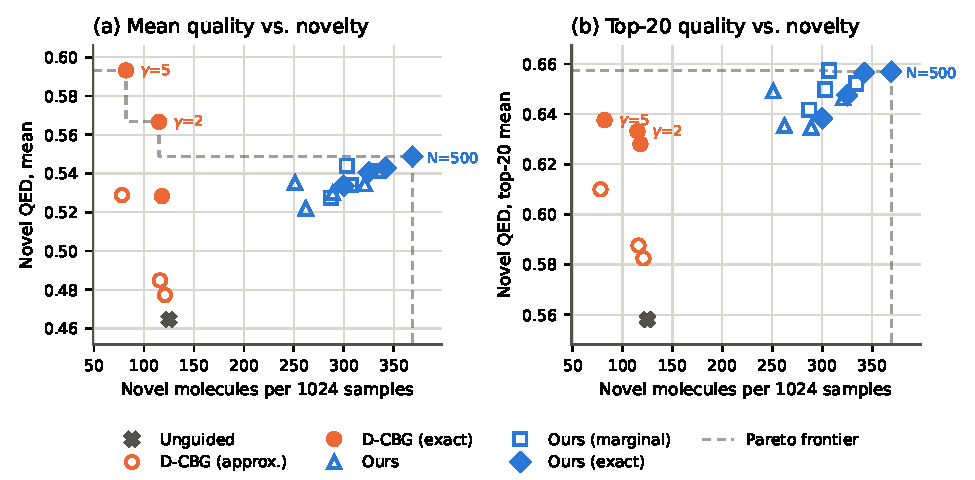
\includegraphics[width=\textwidth]{../figures/pareto_qed.pdf}
\caption{Quality against novelty, all 19 configurations of
Table~\ref{tab:headline}. Panel (a) uses the mean novel QED of that table: the
front holds three points --- D-CBG exact $\gamma = 5$ and $\gamma = 2$, and our
\textbf{exact} $N{=}500$ --- so on the mean neither method dominates and the
choice is a genuine trade-off; note that D-CBG exact $\gamma = 1$ and the whole
approximate branch are dominated by our rows. Panel (b) replaces the mean with
the budget-matched top-20 mean and the picture changes: the front is entirely
ours, every D-CBG configuration is strictly dominated, and $10$ of our $12$
configurations beat $\gamma = 5$ on \emph{both} axes at once (the remaining two
match its top-20 to within $0.003$ with $3.2$--$3.5\times$ the novel count).}
\label{fig:pareto}
\end{figure}

Figure~\ref{fig:pareto} plots the two readings side by side. The mean view (a)
is the one Table~\ref{tab:headline} reports and it shows a real trade-off: the
front runs from D-CBG's high-quality, low-novelty corner to our high-novelty
corner, and picking a point on it is a choice about what the samples are for.
The top-20 view (b) is not a trade-off at all --- our configurations dominate
the D-CBG family outright, since they are better on both axes simultaneously.
The two panels use identical data and differ only in which order statistic of
the same QED distribution is on the $y$ axis, which is the point: the head-to-head
verdict of Section~\ref{sec:headline} is a statement about means, not about
quality.

Figure~\ref{fig:dist} shows the distributions the two summaries come from, and
the two families move differently. For D-CBG the box climbs toward a ceiling that
does not move with it: from $\gamma = 1$ to $\gamma = 5$ the median goes
$0.544 \to 0.600$ while the 95th percentile only goes $0.637 \to 0.648$ and the
99th actually falls, $0.677 \to 0.654$, as does the maximum, $0.689 \to 0.656$.
Guidance strength is buying the middle of the distribution by clipping its
extreme tail. For ours the tail is what moves: from $N = 100$ to $N = 500$ the
95th percentile goes $0.628 \to 0.643$, the 99th $0.652 \to 0.657$, and the
maximum $0.672 \to 0.735$, with the median rising only $0.539 \to 0.550$.

\begin{figure}[h]
\centering
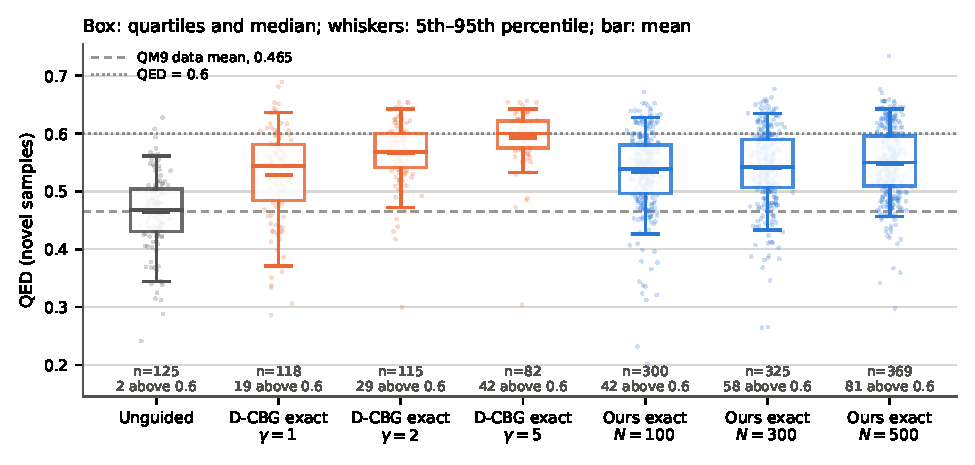
\includegraphics[width=\textwidth]{../figures/novel_qed_dist.pdf}
\caption{Novel QED distributions behind the two means, exact variants only, one
dot per novel molecule. Increasing $\gamma$ (orange) concentrates the
distribution into a band below $0.6$ and shrinks the novel count; increasing $N$
(blue) shifts the distribution up while keeping its spread, so the count above
$0.6$ grows from 42 to 81 even though the mean stays lower.}
\label{fig:dist}
\end{figure}

\paragraph{What this does and does not change.}
It does not overturn Section~\ref{sec:headline}: on the paper's metric --- mean
QED over novel sequences --- exact D-CBG is ahead by $0.044$ and that number
stands. What it changes is the interpretation. The gap is not evidence that
D-CBG's guidance finds better molecules; it is evidence that D-CBG's guidance is
more \emph{aggressive}, moving mass off the low-QED tail at the cost of novelty
and diversity, and a mean rewards exactly that. On any statistic that asks about
the good molecules rather than the average one --- top-20, count above a
threshold, best-of-budget --- the reward-tilted posterior is ahead at the same
sampling cost and with no trained classifier. Both readings are worth reporting,
and a single-number comparison on QED mean is the one that flatters the baseline.

\section{Denoising steps: 32 against 150}
\label{sec:steps}

Every run above fixes \texttt{sampling.steps} $= 32$, the paper's setting. The
step count deserves its own axis because the reward-tilted posterior draws a
fresh set of $N$ candidates and applies the tilt at \emph{every} step, so 150
steps apply it 4.7 times as often at the same $N$; and because \textbf{exact}
commits to one sampled $\mathbf{x}_0$ per step, so more steps means more
commitments but a smaller move per commitment. Table~\ref{tab:steps150} repeats
the two variants at 150 steps, extending $N$ down to 10 and 50, with an unguided
row at the same step count as reference. $T = 0$ (continuous time), so there is
no $t$-grid snapping and 150 steps is well posed. \texttt{aggregate\_x0} and
D-CBG are omitted; D-CBG's exact branch costs about 55 minutes per configuration
at 32 steps and would be roughly 4.3 hours at 150.

\begin{table}[h]
\centering
\caption{150 denoising steps, 1024 samples, seed 1, same UDLM-QM9 base model.
$\Delta$ columns are the change from the matched 32-step row of
Table~\ref{tab:headline}; a dash means Table~\ref{tab:headline} has no such row.
All settings use $\lambda = 5000$ over all $t$ except the last row of each block.}
\label{tab:steps150}
\begin{tabular}{llrrrrrr}
\toprule
Variant & Setting & Valid & Novel & Novel QED & $\Delta$Valid & $\Delta$Novel & $\Delta$NQED \\
\midrule
Unguided & ---                                & 1015 & 165 & 0.459 & $+13$ & $+40$  & $-0.006$ \\
\midrule
exact    & $N{=}10$                            & 995  & 199 & 0.500 & ---   & ---    & ---      \\
exact    & $N{=}50$                            & 1011 & 193 & 0.530 & ---   & ---    & ---      \\
exact    & $N{=}100$                           & 1002 & 208 & 0.531 & $+82$ & $-92$  & $-0.003$ \\
exact    & $N{=}300$                           & 985  & 250 & 0.538 & $+49$ & $-75$  & $-0.003$ \\
exact    & $N{=}500$                           & 994  & 252 & 0.543 & $+73$ & $-117$ & $-0.006$ \\
exact    & $N{=}500$, $\lambda{=}1000$, $t \le 0.75$ & 991 & 280 & 0.536 & $+61$ & $-62$ & $-0.007$ \\
\midrule
marginal & $N{=}10$                            & 992  & 219 & 0.507 & ---   & ---    & ---      \\
marginal & $N{=}50$                            & 1001 & 210 & 0.521 & ---   & ---    & ---      \\
marginal & $N{=}100$                           & 1005 & 222 & 0.534 & $+73$ & $-65$  & $+0.007$ \\
marginal & $N{=}300$                           & 996  & 248 & 0.533 & $+73$ & $-59$  & $-0.001$ \\
marginal & $N{=}500$                           & 984  & 254 & 0.537 & $+69$ & $-80$  & $-0.004$ \\
marginal & $N{=}500$, $\lambda{=}1000$, $t \le 0.75$ & 980 & 236 & 0.534 & $+52$ & $-67$ & $-0.010$ \\
\bottomrule
\end{tabular}
\end{table}

\paragraph{More steps buy validity we did not need and give up the throughput
advantage.}
The direction is the same in all eight matched pairs: validity rises by 49--82
counts, novel counts fall by 59--117, and novel QED moves by at most $\pm 0.010$
with seven of eight pairs flat or slightly negative. Guided validity goes from
89--91\,\% at 32 steps to 96--99\,\% at 150, which closes the gap to
\texttt{aggregate\_x0} and to unguided sampling entirely --- but validity was
never the binding constraint, since novel QED is the reported metric and D-CBG
already matched us there. What is lost is the one axis where we beat D-CBG
outright: our best novel count falls from 369 to 280, against D-CBG's 82. At 4.7
times the sampling cost, 150 steps is a worse operating point for this method,
and 32 steps should stay the default.

\paragraph{The effect is specific to the guided sampler.}
Unguided sampling moves the \emph{opposite} way: 125 novel molecules at 32 steps
against 165 at 150, an increase, while every guided row decreases. So this is not
a generic ``more steps means more memorization'' effect of the base model. The
reading that fits both is that step size, not step count, controls how far
guidance displaces a trajectory. At 32 steps each reverse step is a large move
and the tilt pushes samples well off the model's typical set --- high novelty,
low validity, and the highest novel QED. At 150 steps each move is small, the
tilt displaces less even though it is applied 4.7 times as often, and samples
stay near the typical set --- high validity, low novelty. The net displacement
shrinks as steps grow, which is the same quantity the $\lambda$ sweep below
saturates against.

\paragraph{The exact-versus-marginal ordering washes out.}
At 32 steps \textbf{exact} beat \textbf{marginal} on novel QED in three of four
matched rows by a consistent $+0.007$ to $+0.008$. At 150 steps it wins four of
six but with mixed signs and a mean advantage of about $+0.002$: $-0.007$ at
$N{=}10$, $+0.009$ at $N{=}50$, $-0.003$ at $N{=}100$, $+0.005$ at $N{=}300$,
$+0.006$ at $N{=}500$ and $+0.002$ on the window row. Against a per-cell standard
error near $0.005$ that is a wash. This is consistent with the step-size reading:
the two variants differ only in whether cross-position correlations survive
within a single reverse step, and when each step moves less there is less
correlation to preserve or destroy. The distinction that Section~\ref{sec:method}
establishes as mathematically real is therefore also empirically small whenever
the sampler takes small steps --- which is worth knowing before treating
\textbf{exact} as the variant to standardize on.

\paragraph{The $\lambda$ curve saturates far earlier at 150 steps.}
$\lambda = 5000$ was selected on the 32-step \texttt{aggregate\_x0} grid
(Section~\ref{sec:grid}) and never retuned for either variant or for a different
step count. Table~\ref{tab:lambda150} probes it at 150 steps.

\begin{table}[h]
\centering
\caption{$\lambda$ at 150 steps, \textbf{exact}, $N = 100$, 1024 samples. The
32-step column is the \texttt{aggregate\_x0} grid at the same $N$ (Table
\ref{tab:grid}), which is the only $\lambda$ series available at 32 steps.}
\label{tab:lambda150}
\begin{tabular}{lrrrrr}
\toprule
$\lambda$ & Valid & Unique & Novel & Novel QED & Novel QED (32 steps) \\
\midrule
100  & 1011 & 995 & 211 & 0.524 & ---   \\
200  & ---  & --- & --- & ---   & 0.505 \\
500  & 998  & 963 & 193 & 0.531 & ---   \\
1000 & 998  & 956 & 190 & 0.531 & 0.515 \\
5000 & 1002 & 958 & 208 & 0.531 & 0.522 \\
\bottomrule
\end{tabular}
\end{table}

At 150 steps novel QED is $0.531$ at $\lambda = 500$, $1000$ and $5000$ --- flat
to three decimals --- and only $\lambda = 100$ falls off, to $0.524$. At 32 steps
the same quantity was still climbing at the top of the range ($0.505 \to 0.515
\to 0.522$ for $\lambda = 200 \to 1000 \to 5000$). So $\lambda$ can be cut
tenfold at 150 steps for nothing, but cutting it does not \emph{improve} anything:
the flat region is a plateau, not a peak, and the 32-step choice was not
mistuned. Combined with the previous paragraphs, more steps flatten every knob
this method exposes --- $\lambda$, the variant, and $N$ (novel QED spans
$0.531$--$0.543$ across $N = 100$--$500$ at 150 steps against $0.534$--$0.549$ at
32). The method has more headroom at coarse discretization, not less.

\paragraph{What this axis does not settle.}
There is no $\lambda = 0$ control at 150 steps. At 32 steps that row showed
\textbf{exact} sampling the true reverse step at 66.3\,\% validity against
97.9\,\% for the factorized base sampler, and the tilt recovering 23.5 of the
31.6 lost points. Whether the 31.6-point gap itself shrinks with step size --- it
should, if step size is what governs displacement --- is untested, and one
5-minute run would answer it.

\section{Why the novel mean is the metric that matters}
\label{sec:novel}

QED (Bickerton et al., 2012) is a weighted geometric mean of eight desirability
functions over molecular weight, ALOGP, hydrogen-bond donors and acceptors,
polar surface area, rotatable bonds, aromatic rings, and structural alerts. Its
molecular-weight term peaks near 300\,Da, whereas QM9 molecules have at most
nine heavy atoms ($\approx$100--150\,Da), so QM9 sits at 0.465 largely because
its molecules are too small to score well. Raising QED on this dataset means
generating larger, more complex molecules, which is also why validity falls as
QED rises.

The valid set decomposes into molecules already present in QM9 and genuinely
novel ones, and the two have systematically different QED. Splitting the
generated samples accordingly:

\begin{table}[h]
\centering
\caption{QED decomposed over the valid set. \emph{Memorized} are valid samples
already in QM9; \emph{novel} are the rest. 1024 samples each. The gap between
the two columns is what separates recall from generalization.}
\label{tab:novel}
\begin{tabular}{lrrrrrr}
\toprule
Run & Valid & Novel & QED (all) & QED memorized & QED novel & Gap \\
\midrule
Unguided                                   & 1002 & 125 & 0.471 & 0.471 & 0.465 & 0.007 \\
D-CBG approx., $\gamma = 5$                & 856  & 78  & 0.556 & 0.558 & 0.529 & \textbf{0.030} \\
D-CBG exact, $\gamma = 1$                  & 949  & 118 & 0.542 & 0.544 & 0.528 & 0.016 \\
D-CBG exact, $\gamma = 2$                  & 903  & 115 & 0.581 & 0.583 & 0.567 & 0.016 \\
D-CBG exact, $\gamma = 5$                  & 968  & 82  & 0.600 & 0.600 & 0.593 & 0.007 \\
Ours $N{=}500$, $\lambda{=}1000$, $t \le 0.75$ & 946 & 251 & 0.540 & 0.541 & 0.535 & \textbf{0.006} \\
Ours $N{=}500$, $\lambda{=}5000$           & 949  & 321 & 0.542 & 0.545 & 0.534 & 0.010 \\
\bottomrule
\end{tabular}
\end{table}

Memorized molecules score higher than novel ones in every run, which is why the
all-valid mean always exceeds the novel mean: the valid set is 75--90\,\%
memorized, so the overall average is pulled toward it. Memorized molecules are
real QM9 entries --- curated, well-formed chemistry --- while the novel ones are
the model's extrapolation, valid but less clean. (The duplicate-versus-set
asymmetry in how the repository computes the two columns is \emph{not} the
cause: recomputing the novel mean with duplicates retained changes it by at most
0.002, since uniqueness runs 92--99\,\%.)

The gap is small and similar for most methods, with one exception: the
\emph{approximate} D-CBG branch at $\gamma = 5$ has a gap of 0.030, four to five
times everyone else's. Its memorized samples average 0.558 while its novel ones
fall to 0.529, meaning much of what the first-order approximation buys is
recovery of high-QED molecules already in the training set rather than new
chemistry. The exact branch does not share this pathology --- its gap at
$\gamma = 5$ is 0.007, the same as unguided and as ours --- so this is a
property of the Taylor approximation, not of classifier guidance as such. An
earlier version of this note generalized the approximate branch's behaviour to
D-CBG in general; that was wrong.

What survives is the count. At $\gamma = 5$ both D-CBG branches produce
\emph{fewer} novel molecules than unguided sampling (82 and 78 against 125),
while our method produces 251--321. So the methods differ less in the quality of
the novel molecules they make than in how many they make at all.

The decomposition also explains why the paper reports the novel mean rather than
the overall mean: the overall mean is contaminated by how well a method
retrieves memorized high-property molecules, while the novel mean measures
whether guidance actually creates new ones.

\section{The guidance time window}
\label{sec:window}

Table~\ref{tab:window} restricts guidance to a sub-range of $t$, which counts
down from 1 (pure noise) to 0 (clean). Outside the window the sampler falls back
exactly to the base model and skips the reward calls entirely.

\begin{table}[h]
\centering
\caption{Guidance time window, $\lambda = 1000$, 1024 samples. $t \le 0.75$
means guidance is off for the 8 noisiest steps of 32; $t \ge 0.5$ means it is
active \emph{only} for those early steps.}
\label{tab:window}
\begin{tabular}{lrrrr rrrr}
\toprule
& \multicolumn{4}{c}{$N = 300$} & \multicolumn{4}{c}{$N = 500$} \\
\cmidrule(lr){2-5}\cmidrule(lr){6-9}
Window & Valid & Novel & QED & Novel QED & Valid & Novel & QED & Novel QED \\
\midrule
all $t$          & 944 & 229 & 0.535 & 0.526 & 967 & 276 & 0.538 & 0.530 \\
$t \le 0.75$     & 955 & 248 & 0.535 & \textbf{0.532} & 946 & 251 & 0.540 & \textbf{0.535} \\
$t \le 0.5$      & 960 & 223 & 0.536 & 0.531 & 973 & 272 & 0.536 & 0.530 \\
$t \le 0.25$     & 961 & 260 & 0.532 & 0.517 & 969 & 266 & 0.531 & 0.528 \\
\midrule
$0.25 \le t \le 0.75$ & 993 & 145 & 0.491 & 0.466 & 993 & 143 & 0.490 & 0.481 \\
$t \ge 0.25$     & 976 & 128 & 0.491 & 0.472 & 979 & 126 & 0.491 & 0.476 \\
$t \ge 0.5$      & 995 & 141 & 0.474 & 0.463 & 991 & 145 & 0.478 & 0.464 \\
\bottomrule
\end{tabular}
\end{table}

The hypothesis that guidance is wasted on the early high-noise steps is
confirmed, and more strongly than expected. Guidance restricted to the early
steps ($t \ge 0.5$) produces novel QED $0.463$--$0.464$, statistically
indistinguishable from the unguided $0.465$: it does \emph{nothing}. The entire
effect comes from the low-noise steps, which is what the mechanism predicts ---
at large $t$ the decoded $\mathbf{x}_0$ candidates are mostly unparseable, so
they all collapse to the invalid reward and the weights go uniform.

Conversely, dropping the noisiest steps is free or mildly beneficial:
$t \le 0.75$ is the best cell for both $N$ values. Even $t \le 0.25$, which runs
the reward on only the last 8 of 32 steps, retains most of the gain
($0.528$ at $N = 500$) at a quarter of the reward cost. This is the practical
recommendation: restrict guidance to $t \lesssim 0.75$, and use $t \le 0.25$ if
throughput matters.

\section{The atomic-measure limitation}
\label{sec:support}

The self-normalized estimator replaces $q(\mathbf{x}_0 \mid \mathbf{x}_t)$ with
an atomic measure supported on exactly $N$ points,
$\hat{q} = \sum_n w_n \delta_{\mathbf{x}_0^{(n)}}$. Under
\texttt{aggregate\_x0} the per-position histogram is
\begin{equation}
\bar{\mathbf{x}}_0^{\,l}[k]
  = \sum_{n=1}^{N} w_n \, \mathbf{1}\{\mathbf{x}_0^{(n),l} = k\},
\end{equation}
so a token $k$ that appears at position $l$ in \emph{none} of the $N$
candidates receives exactly zero mass. The method is therefore an implicit
\emph{stochastic truncation} of the denoiser: since the candidates are drawn
i.i.d.\ from $p_\theta(\mathbf{x}_0^l \mid \mathbf{x}_t)$, a token survives with
probability $1 - (1 - p)^N$, so tokens with $p \ll 1/N$ are dropped almost
surely. With the 40-token QM9 SMILES vocabulary and $N = 100$, this suppresses
everything below roughly the 1\,\% tail.

For uniform diffusion the suppression is severe but not absolute: the posterior
in \texttt{diffusion.py} contains a term
$(1 - \alpha_{ts})(1 - \alpha_s)\,\pi_{\text{limit}}$ that is positive for every
token independently of $\bar{\mathbf{x}}_0$, so unseen tokens retain a small
uniform floor --- one to two orders of magnitude below an observed token at
these step sizes. For absorbing-state diffusion the posterior is
$\bar{\mathbf{x}}_0(\text{move}_t - \text{move}_s)$ with the mask term added
separately, and unseen tokens are \emph{exactly} zero.

This is plausibly what caps the achievable property gain, and it cuts both
ways: truncating the tail is also the most likely reason validity \emph{rises}
under guidance (94--98\,\% against 97.9\,\% unguided) while novelty falls, since
suppressing low-probability tokens removes both malformed strings and unusual
but legitimate ones. The \texttt{support\_floor} option tests this directly by
mixing the denoiser marginal back in,
\begin{equation}
\bar{\mathbf{x}}_0 \leftarrow
  \frac{\bar{\mathbf{x}}_0 + \epsilon\, \mathbf{x}_\theta}{1 + \epsilon},
\end{equation}
which restores full support for any $\epsilon > 0$ while leaving the tilt
intact; $\epsilon = 0$ recovers the plain estimator.

\paragraph{The fix makes things worse.}
Measured at $N = 300$, $\lambda = 1000$, 1024 samples, the floor destroys the
gain rather than extending it:

\begin{center}
\begin{tabular}{lrrrr}
\toprule
$\epsilon$ & Valid & Novel & QED mean & Novel QED \\
\midrule
0 (none) & 944 & 229 & 0.535 & \textbf{0.526} \\
0.01     & 965 & 113 & 0.508 & 0.481 \\
0.1      & 988 & 120 & 0.492 & 0.480 \\
0.5      & 993 & 113 & 0.479 & 0.474 \\
\bottomrule
\end{tabular}
\end{center}

Even $\epsilon = 0.01$ gives back most of the improvement, and the novel count
halves. The reason is that the mixture is applied per position and per step:
where the weighted histogram is nearly one-hot, adding $\epsilon\,
\mathbf{x}_\theta$ injects an $\epsilon$ chance of an off-distribution token at
each of the 32 positions on each of the 32 steps, so on the order of
$\epsilon \cdot 32 \cdot 32 \approx 10$ tokens get resampled from the untilted
model over a trajectory. That is enough to walk the sample back toward
$p_\theta$.

The conclusion is the opposite of the initial worry: the atomic truncation is
not a defect limiting the method, it is part of why the method works. Restricting
the reverse step to tokens that at least one high-reward candidate proposed acts
like nucleus sampling with a $1/N$ threshold, which is also the most plausible
explanation for validity holding at 94--97\,\% under guidance. Support should be
widened by raising $N$ --- which draws more atoms from the correct tilted region
--- not by blending in the untilted marginal.

\paragraph{A note on combining with D-CBG.}
The two mechanisms act on different objects and look complementary. D-CBG
reshapes the \emph{proposal} through per-token classifier gradients, and our
method reweights \emph{whole-sequence} candidates with an exact reward. Drawing
the $N$ candidates from a D-CBG-tilted proposal
$\tilde{p}_\theta(\mathbf{x}_0 \mid \mathbf{x}_t)$ and then reweighting with
$w_n \propto \exp(\lambda r(\mathbf{x}_0^{(n)}))\,
p_\theta(\mathbf{x}_0^{(n)})/\tilde{p}_\theta(\mathbf{x}_0^{(n)})$ --- both
densities being explicit, so the correction is computable --- would attack
exactly the limitation above, because the atoms would land where the reward is
already high instead of where the untilted model happens to sample. Not
implemented; recorded here as a direction.

\section{Pending runs}
\label{sec:pending}

The UDLM axis above is complete at both 32 and 150 steps
(Section~\ref{sec:steps}), with one gap noted there: no $\lambda = 0$ control at
150 steps. The MDLM (absorbing-state) axis is in progress:
both prerequisites finished training for 25k steps --- an MDLM generative model
(DiT-small, since no MDLM-QM9 checkpoint is published; the released MDLM models
are all OpenWebText with a 1024-token GPT-2 vocabulary) and an absorbing-state
D-CBG classifier. The comparison sweep is running.

Early MDLM numbers at 1024 samples: unguided gives novel QED 0.461 with only
64.8\,\% validity, and our method at $N = 100$ reaches 0.499--0.500. The low
validity reflects that this MDLM is a from-scratch 25k-step model rather than a
released checkpoint, so it is a weaker base than the HuggingFace UDLM; its
novelty is correspondingly much higher (47\,\% of valid against 12\,\% for
UDLM), meaning it memorizes far less. Cross-model comparisons of absolute
numbers are therefore not meaningful --- only the within-model deltas are.

MDLM remains the sharper test of Section~\ref{sec:support}: its posterior has no
uniform floor, so tokens no candidate proposed are \emph{exactly} zero rather
than merely suppressed, and \texttt{aggregate\_x0} coincides exactly with
\texttt{marginal}. The sweep includes the same \texttt{support\_floor} ablation
for that reason.

The clearest remaining gap is \textbf{exact} on MDLM. The
\texttt{mixture\_sampling=exact} runs reported in Table~\ref{tab:headline} are
UDLM only, and \texttt{scripts/server\_run\_comparison\_mdlm.sh} fixes
\texttt{aggregate\_x0}; since \textbf{exact} on masked diffusion is precisely
EDLM's Algorithm 1 with the energy swapped for a reward, that cell is the direct
test of the substitution in the setting EDLM itself used. Note that
\texttt{aggregate\_x0} and \texttt{marginal} coincide there, so MDLM has only two
distinct variants and \textbf{exact} is the one that matters. The $\lambda$ that
worked on UDLM will not transfer --- the tilt has to be recalibrated against the
weaker base model's reward scale, watching ESS.
Regenerate the combined table with
\begin{verbatim}
rsync -av wp03052@143.248.84.179:~/Synthetic-Data/Molecule/results/ ./results/
python scripts/make_results_table.py results pdfs
\end{verbatim}
which writes \texttt{pdfs/sweep\_table.tex} and \texttt{pdfs/sweep\_table.md}.

\section{Reproducing}

\begin{verbatim}
# our method
python guidance_eval/our_qm9_eval.py \
  data=qm9 data.label_col=qed \
  backbone=hf_dit model=hf model.length=32 \
  model.pretrained_model_name_or_path=kuleshov-group/udlm-qm9 \
  diffusion=uniform parameterization=d3pm \
  time_conditioning=True zero_recon_loss=True \
  guidance=ours guidance.reward=qed guidance.lambda_=50 \
  guidance.mixture_sampling=aggregate_x0 guidance.num_x0_samples=30 \
  guidance.t_min=0.0 guidance.t_max=0.5 \
  sampling.steps=32 sampling.num_sample_batches=8 sampling.batch_size=64 \
  sampling.use_cache=False eval.disable_ema=True

# full sweep + D-CBG baseline (inside tmux)
bash scripts/server_train_cbg_classifier.sh uniform qed
bash scripts/server_run_comparison.sh
\end{verbatim}

Implementation lives in \texttt{our\_guidance.py} and
\texttt{configs/guidance/ours.yaml}; nothing in the original repository was
modified.

\end{document}
